\section{Colour Theory}
\label{research:ColourTheory}
Diving into some research about colour theory I have looked at the various styles artists and company use to represent ideas and feelings to the user
\begin{figure}[H]
    \centering
    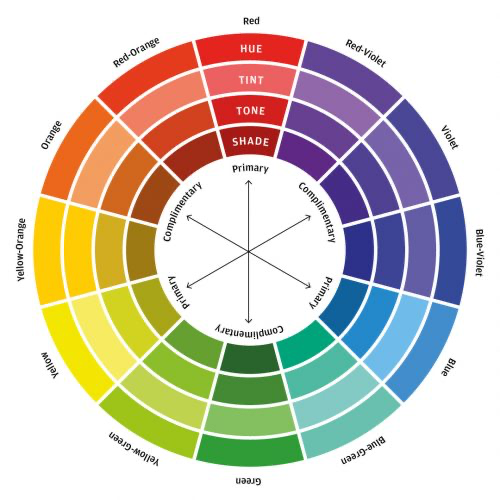
\includegraphics[width=0.5\textwidth]{Research/6_ColourTheory/media/ColourWheel.png}
    \caption{The colour wheel, illustrating primary, secondary, and tertiary colours.}
    \label{fig:colourwheel}
\end{figure}

This colour wheel summarises my learnings about hue, tone, shade and tint nicely with visual examples. Although some uses of monocolour design can appear lifeless, the clever use of shades can really make a design pop and be visually appealing

\begin{figure}[H]
    \centering
    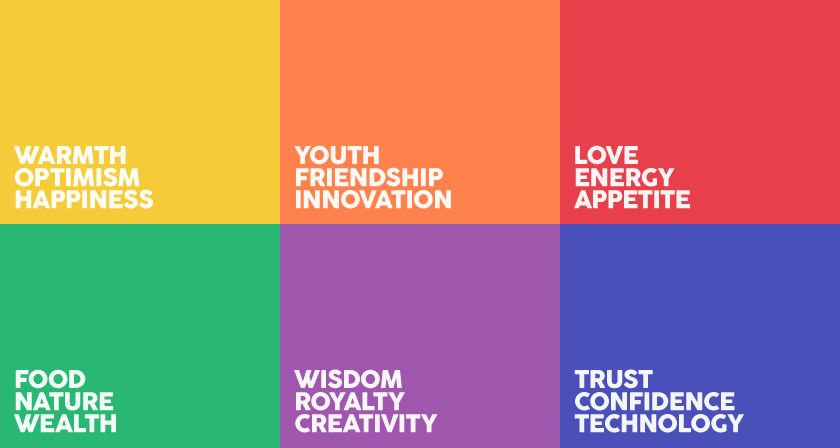
\includegraphics[width=0.5\textwidth]{Research/6_ColourTheory/media/MoodChart.png}
    \caption{A Moodchart showcasing the various emotions and feelings associated with different colours.}
    \label{fig:colourpalette}
\end{figure}
The ideas of wisdom, creativity, trust and confidence underpin the goals of my EPQ. These colours naturally fit my vision perfectly and, alongside being my favourite colours will be the primary tones in my ui designs


Further expanding on purple/blue shades I used an online tool to help me curate colour palettes for use in my designs. The second (more pastel) palette really draws my eye
\begin{figure}[H]
    \centering
    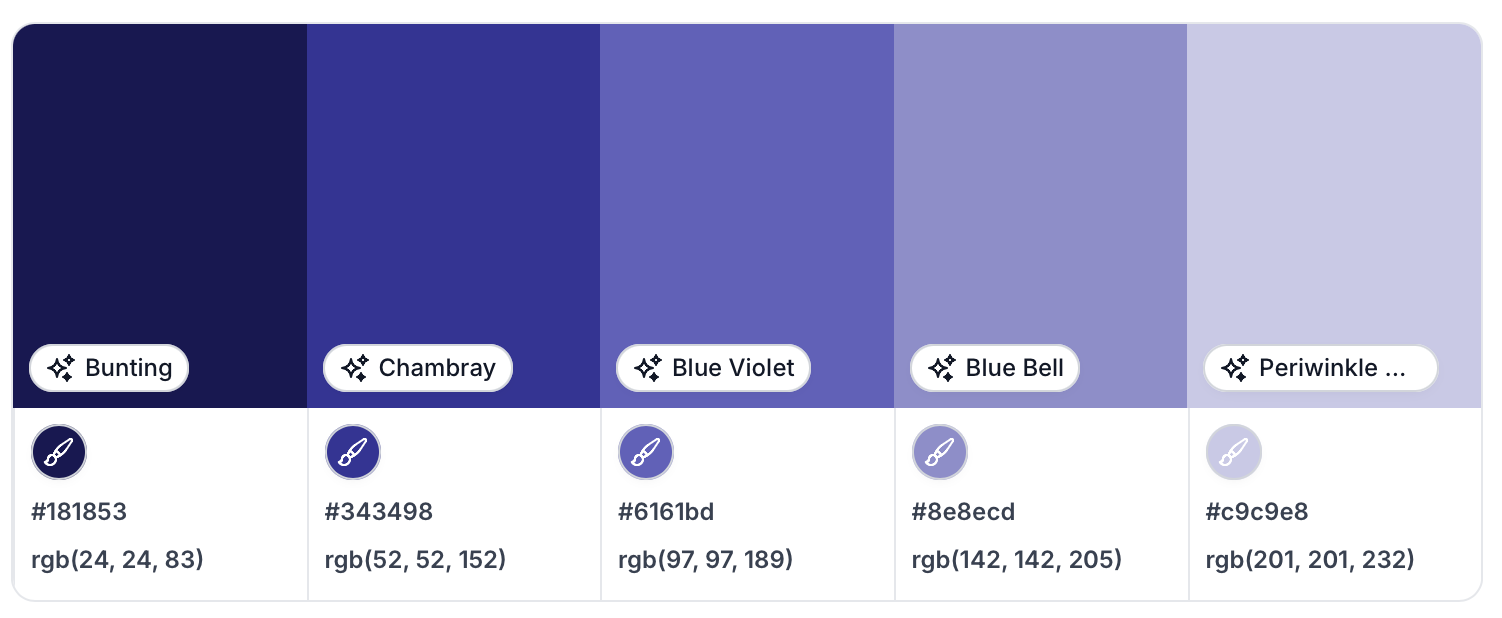
\includegraphics[width=0.5\textwidth]{Research/6_ColourTheory/media/Pallete1.png}
    \caption{1st Colour Palette}
    \label{fig:colourpalette1}
\end{figure}
\begin{figure}[H]
    \centering
    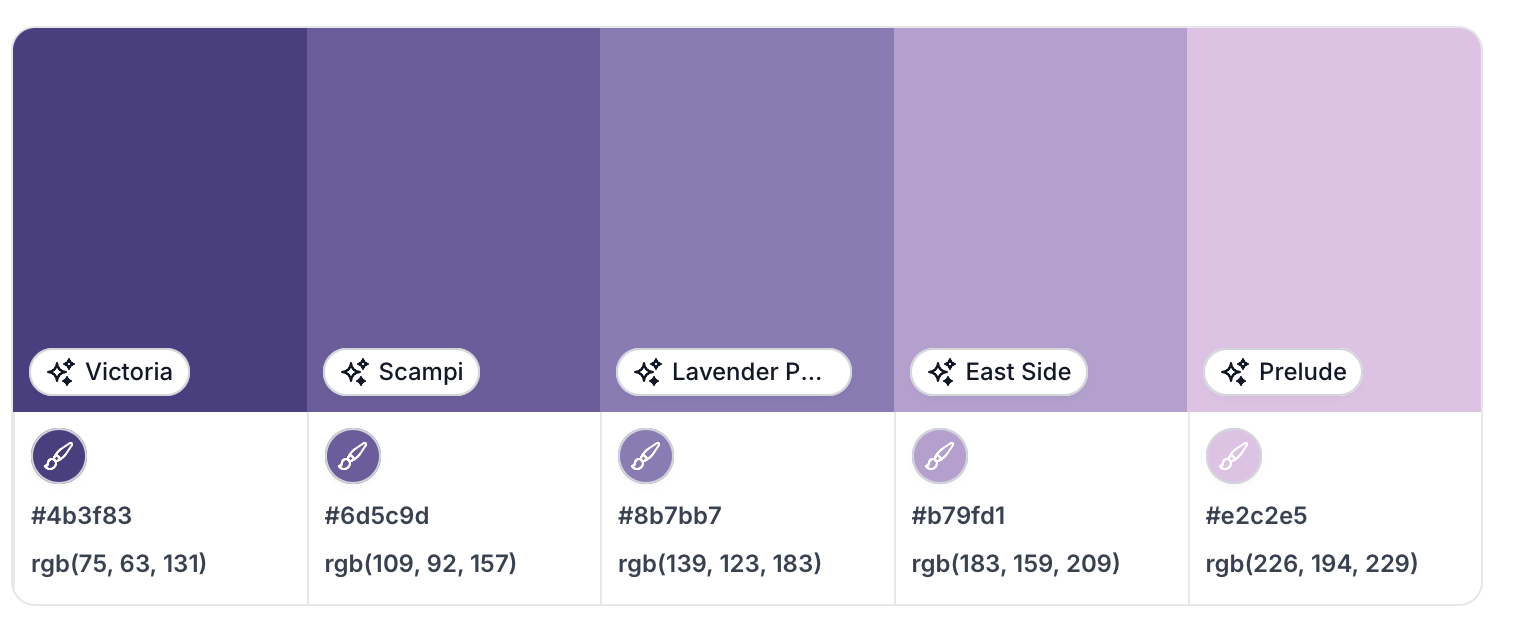
\includegraphics[width=0.5\textwidth]{Research/6_ColourTheory/media/Pallete2.png}
    \caption{2nd Colour Palette}
    \label{fig:colourpalette2}
\end{figure}

With a greater idea on the colours i wanted to use i explored existing interfaces to see how the designers merged the colours into their designs.
\begin{figure}[H]
    \centering
    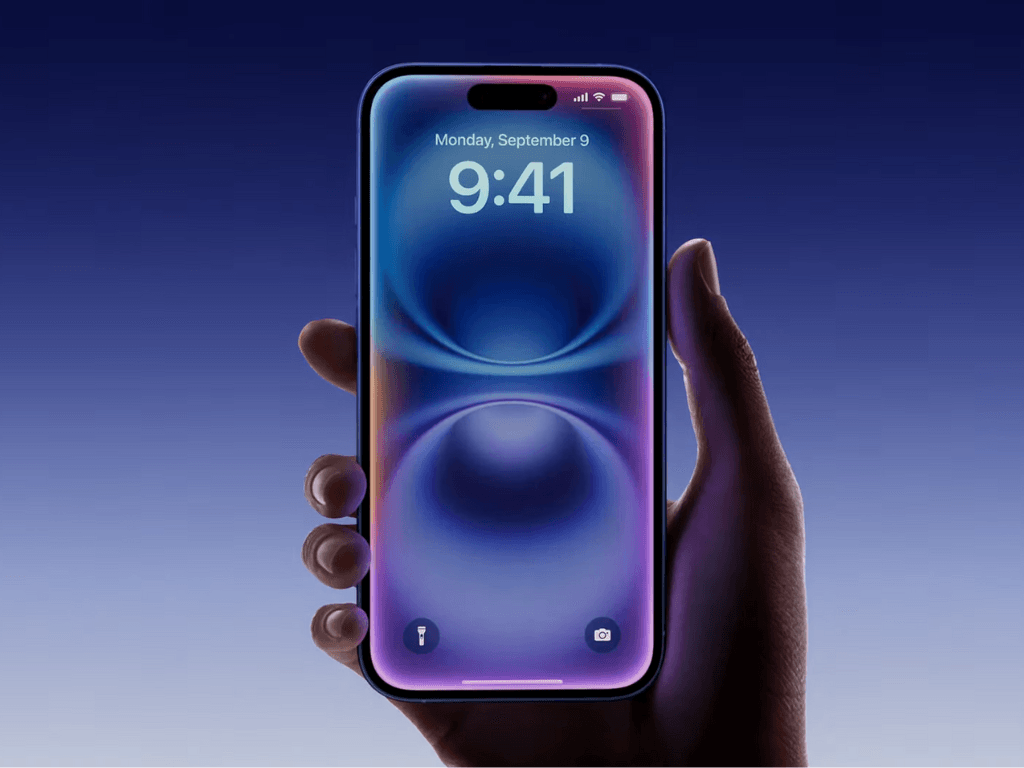
\includegraphics[width=0.5\textwidth]{Research/6_ColourTheory/media/Apple.png}
    \caption{Apple's use of colour in their AI Siri interface design.}
    \label{fig:colourexample1}
\end{figure}
I saw this Apple AI demo video, and this frame in particular caught my interest as the glowing, pulsing colour border really draws the eye, this design signals life and gives confidence In the machines "thought" process. I really want to learn from this and incorporate similar ideas in my artifact.
\begin{figure}[H]
    \centering
    
\includegraphics[width=0.5\textwidth]{Research/6_ColourTheory/media/Waves.png}
    \caption{Wave wallpaper.}
    \label{fig:colourexample2}
\end{figure}
This Gradient wallpaper nicely demonstrates the impact a few well thought out colour tones can have.

